\documentclass[letterpaper,twocolumn,10pt]{article}
\usepackage{usenix,epsfig,endnotes}
\usepackage{float}
\usepackage{subfigure}
\usepackage{algorithm} %format of the algorithm
\usepackage{algorithmic} %format of the algorithm
\usepackage{multirow} %multirow for format of table
\usepackage{amsmath}
\usepackage{xcolor}
\usepackage{url}
\usepackage{hyperref}
\usepackage{breakurl}
\usepackage{xspace}
\usepackage{flushend}
%\usepackage{Utopia}

\renewcommand{\algorithmicrequire}{\textbf{Input:}}
\renewcommand{\algorithmicensure}{\textbf{Output:}}



\newcommand\LSMForest{{LSM-Forest}\xspace}
\hyphenation{LSM-Forest}

\newcommand\DBC{Distributed BloomCluster\xspace}
\newcommand\DBCs{DBC\xspace}
\newcommand\DBCss{DBCs\xspace}


\begin{document}

%don't want date printed
\date{}


\title{Title}

\author{
    Author1, 
    Author2, 
    Author3,
    Author4,
    Author5
} % end author


\maketitle
\section{Introduction}
\label{sec-1}

To be finished.
\section{Trace data and Analysis Methodology}

\subsection{System structure}
\label{sec2.1}
The system provides services to users in the form of cloud disk. Users can use cloud disk in a manner similar to local disk, for example, as a system disk or data disk. In the system, each cloud disk segment is divided into fixed-size segments (32GB). The system is divided into several clusters. The architecture of the cluster is shown in figure 1, and the overall architecture is shown in figure 2. The bottom layer of each cluster is an append-only distributed file system. The Block service layer abstracts the append-only files into fixed-size blocks for users by means of log-structure-merge. The Block server is responsible for pulling the segment metadata and passing the data between users and segments in a proxy manner. All read and write traffic to segment goes through the corresponding block server. The master node stores the block server information corresponding to the segment and provides control services for the block server, such as the addition, deletion and error recovery of the block server. 


\subsection{Existing Problems}
\label{sec2.2}
As cloud computing becomes more widely used, more and more users are deploying their services on the cloud. These users run different types of services, while these services may access cloud disk in very different manner. Using simple rules to place cloud disk may lead to serious load skew between different block servers, so that network resources cannot be fully utilized. Users sending read and write requests to high-load block server will feel serious tail delay, which will affect user experience.
% As is known to all, the throughput of each device, or rather, each segment varies greatly with time. In the current structure, the throughput of block servers may be imbalanced after a period of time without rebalacing. The imbalance will lead to the following consequences: 

% \begin{itemize}
%     \item Some block servers may reach the maximum throughput. Cloud disk application providers have to add new servers even new clusters;
%     \item Long tail effect may appear, i.e., some devices may suffer from high latency and slow reads and writes.
% \end{itemize}

% In summary, analyses of I/O pattern of cloud disks and efforts to improve the situation are necessary.

\subsection{Analysis Methods}
\label{sec2.3}
In order to solve the load skew problem of the block service layer, we conducted a statistical analysis on the trace of the online system to evaluate the impact of different cloud disk access characteristics on cluster load balancing.
\begin{table}[ht]
    \footnotesize
    \centering
    \begin{tabular}{c|c|c|c|c}
         Cluster & Number of BS & Number of disk & Type & Capacity\\
         AY306L & 48 & 2559 & ESSD & 846699G\\
         AY251Z & 96 & 4696 & ESSD & 1629415G\\
         AY272T & 82 & 8552 & SSD & 1523944G\\
         AY306O & 95 & 26297 & Efficient & 3048367G\\
         AY336D & 96 & 33154 & Efficient & 3062493G\\
         AY272M & 95 & 32719 & Efficient & 3438001G\\
    \end{tabular}
    \caption{Trace Data Attributes}
    \label{table2.3-1}
\end{table}
The details of Trace are shown in Table \ref{table2.3-1}. Trace records the read and write traffic of all segments at different times, with minute granularity, and indicates the block server where the segment is located. We conducted a multidimensional analysis of trace. By observing the load balance of different clusters and the distribution of cloud disk features. We find some key factors.
At the same time,we use a scheduling simulator is to evaluate the effcet of different placement strategies and scheduling algorithms.
% Since the current situation is not good enough, we need to analyse the trace as well as schedule the cluster to improve the situation. We use a simulator to simulate the scheduling process and output the schedule result.

In order to analyse if the scheduling strategy is good, we need to define an index to measure the level of load balance. Here we choose the variance of read throughput between block servers as a measurement. As the variance changes over time, we use median of variances over time as a measurement when we want to judge the schedule effect over a period of time. Due to the fact that the movement of a segment employs computation resource as well as time, we define the number of moving as the schedule cost. Thus, the target of rebalance is to minimize read throughput and schedule cost.

% \subsection{Trace Data}
% \label{sec2.4}
% We use trace of clusters in business environment for simulation. We select 6 clusters, including ESSD clusters, SSD clusters and efficient clusters in a certain available zone for analysis. Since there are clusters with all levels of performance, the analysis is comprehensive.

% Considering the size of data set and simulation efficiency, the grain fineness of trace data is 1 minute, i.e., we can know the read and write throughput per minute from the trace data. If the time range of trace data is too long, analysis will be difficult. Thus, we select a representative time range, which is from 2020-2-10 17:00 to 2020-2-10 19:00 (UTC+8:00). 

% Each item of trace data includes six fields: time, device, segment, read throughput, write throughput and host. These data are sufficient for analysis and scheduling simulation.

\section{Analysis}
\subsection{Trace analysis}
\label{sec3.1-0}

In this chapter, we mainly introduce some phenomena and understandings observed through trace analysis. Since the average write traffic of the cluster in trace is much higher than the read traffic, we believe that the write traffic in the cloud environment is a more scarce resource. Therefore, the following paper explores the load balancing problem centering on the write traffic.

\subsubsection{Unbalanced network traffic distribution} 
\label{sec3.1-1}
\begin{table}[ht]
    %\footnotesize
    \small
    \centering
    \begin{tabular}{c|c|c}
         Cluster &Block server&Write traffic\\
         AY306L & 48 & 1.03E+13 \\
         AY251Z & 96 & 1.99E+13 \\
         AY272T & 82 & 2.35E+13 \\
         AY306O & 95 & 1.90E+13 \\
         AY336D & 96 & 2.05E+13 \\
         AY272M & 95 & 1.99E+13 \\
    \end{tabular}
    \caption{Cumulative write traffic}
    \label{table3.1-1}
\end{table}
\begin{figure}[ht]
    \centering
    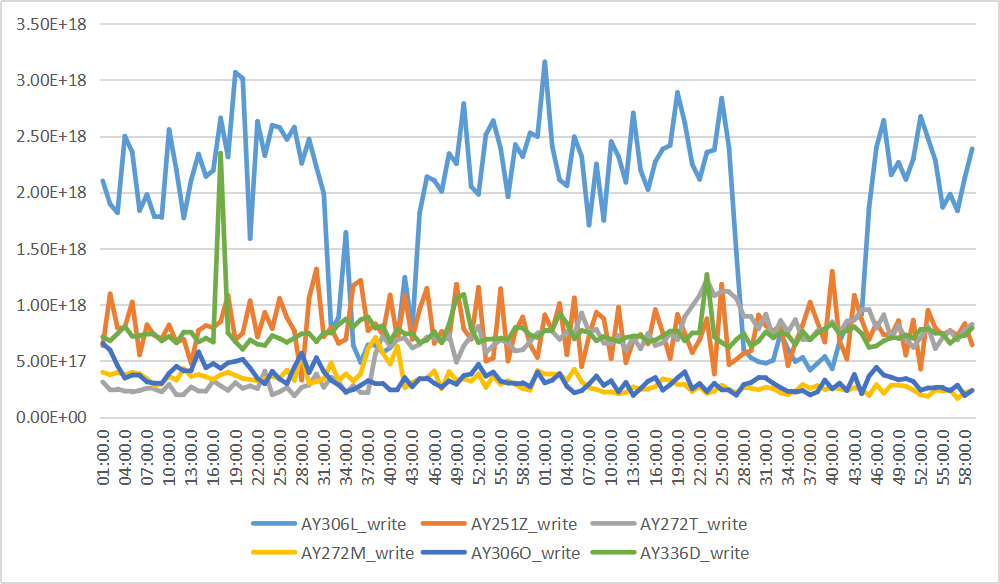
\includegraphics[width=0.4\textwidth]{Figure-3.1/Figure_3-1.png}
    \caption{Unbalance in different clusters}
    \label{fig3-1}
\end{figure}
We made a statistical analysis on the access and load balancing of the six clusters. First, we counted the cumulative write traffic of the six clusters in trace for two hours(Table \ref{table3.1-1}). We then calculated the variance of write traffic of different block servers in each cluster(Figure \ref{fig3-1}).Tthe vertical axis is the traffic variance of block server in the cluster, and the horizontal axis is the time, a serious imbalance can be obeserved.



\subsubsection{Impact of Group User}
\label{sec3.1-2}
First, we counted the cumulative traffic distribution in the segment. We observed that cloud disk of the same user may be similar in the write traffic characteristics. When the user scale is large and cloud disk has a large write traffic, it may have a great impact on the overall balance degree of the cluster. This kind of phenomenon appear in cluster AY272T and AY336D, their segment accumulated traffic and block server cumulative traffic as shown in figure,we can observe the four highest traffic segment belong to the same cloud disk, and their write traffic is very high, the cloud disk flow curve as shown in figure,It can be found that it is similar to the cluster balance degree curve characteristics, so it can be inferred that the balance degree fluctuation of cluster AY306L is affected by the cloud disk.


\subsubsection{Write Traffic Distribution of Segments}
\label{sec3.1-3}
First we delete cluster AY272T, AY336D from Figure \ref{fig3-1} to eliminate impact of group user.The write traffic variance of ESSD in the figure is greater than that of efficient disk. Based on this observation, we guess the cluster's traffic balance degree may be associated with the cloud disk performance, namely the high performance disk is more likely to cause imbalance phenomenon.

We observed the changes of block server traffic in different clusters and found that most of the write traffic fluctuations of block servers are not very large, but there are significant differences among different block servers(Figure \ref{fig3-2}).Occasionally there is a large fluctuation, but it is affected by  few segments of very high write traffic disk.Therefore, we assume that the segment traffic distribution is unbalanced, and this imbalance leads to traffic differences between block servers.To confirm our hypothesis,we calculated the cumulative write traffic of all segments(Figure \ref{fig3-3}), which is like the zipF distribution.Basically The top 10\% segments add up to 80\% of the total traffic.


Since the traffic difference between different segments may be large, the cluster balance degree is mainly affected by a small part of segments with higher traffic ranking.In order to observe the proportion and distribution of these segments in different clusters, we intercepted the segments whose cumulative traffic was greater than 1/10 of the average traffic of block servers for observation(Figure \ref{fig3-4}).
\begin{figure}[ht]
    \centering
    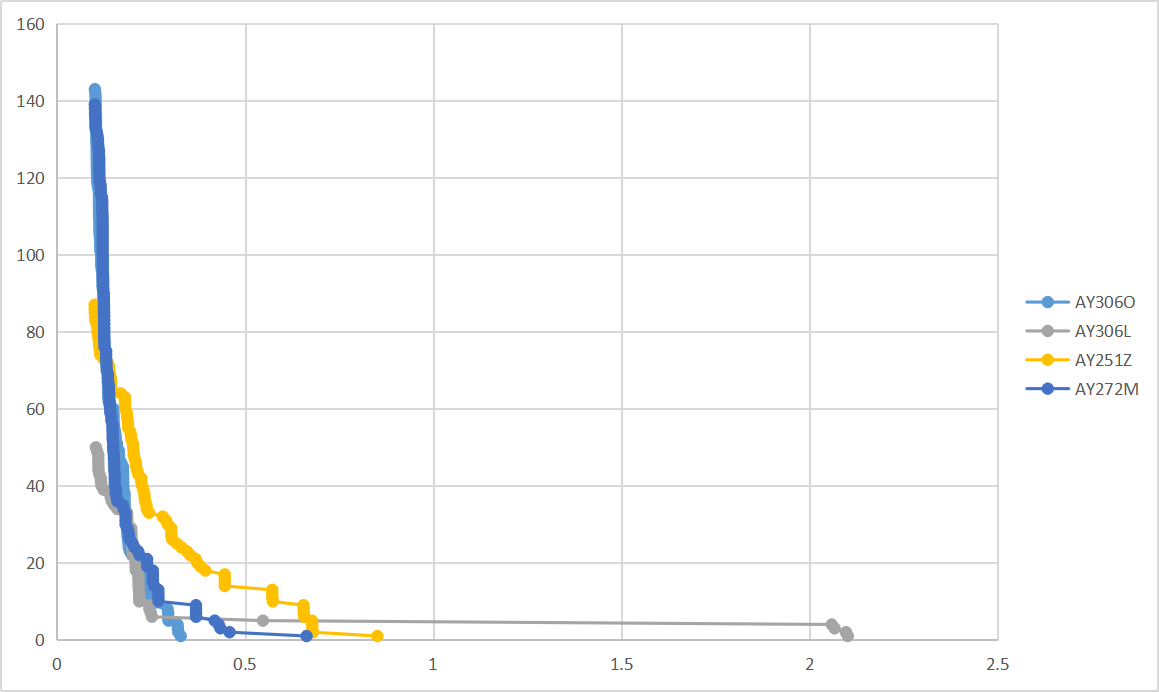
\includegraphics[width=0.4\textwidth]{Figure-3.1/Figure_3-3.png}
    \caption{Segment traffic distribution of different clusters}
    \label{fig3-4}
\end{figure}
(Figure \ref{fig3-4}).
It can be found that the curve of the high-performance disk approaches 0 at a slower speed, which indicates Among the few segments with the highest network traffic 
1. High performance clusters have higher peaks
2. High performance clusters Large degree of dispersion
As a result, the placement of these segments is more likely to cause imbalance
\subsection{Impact of Simple Scheduling Strategies}
\label{sec3.2-0}

In this section, we introduce a simple segment-based balancing method based on historical records and greedy strategy, which move segments periodically to rebalance the throughput of block servers. Moreover, the influence of different parameters on the scheduling results will be analyzed.

\subsubsection{Introduction to Simple Scheduling Strategies} 
\label{sec3.2-1}

We first define a \textit{simple greedy strategy}, which performs a round of schedule at a specified time interval (to be specified by the administrator). When the time to schedule arrives, the scheduler will calculate the historical average on every segment over a period of time. Then, the scheduler will traverse segments by historical records from high to low. The scheduler will move the segment to the block server which has the lowest throughput. Obviously, schedule frequency and the time length of historical record will make an impact on the schedule result.

In the sections below, we will discuss the impact of several parameters (e.g. knowledge of future throughput, proportion of scheduling segments). All these topics will be discussed on the \textit{simple greedy strategy} as an example.


\subsubsection{Impact of Greedy Algorithm}
\label{sec3.2-2}

We simulate simple greedy algorithm on different clusters. We can find that simple greedy strategy can reduce the variance in some degree, but there's still some distance to the upper limit (Table \ref{table3.2-1}). What's worse, sometimes, negative optimizations may occur (Figure \ref{fig3.2-1}). The reason is that average of historical records can not describe the pattern of the cluster properly. 

\begin{table}[ht]
    \footnotesize
    \centering
    \begin{tabular}{c|c|c|c|c}
         Cluster & Type& No Schedule & Greedy & Future\\
         AY306L & ESSD & 2.13E+18 & 6.51E+17 & 5.36E+17\\
         AY251Z & ESSD & 7.68E+17 & 5.53E+17 & 1.99E+17\\
         AY272T & SSD & 6.87E+17 & 1.10E+17 & 3.02E+16\\
         AY306O & Efficient & 3.08E+17 & 1.14E+17 & 3.29E+06\\
         AY336D & Efficient & 7.27E+17 & 1.12E+17 & 3.35E+06\\
         AY272M & Efficient & 2.97E+17 & 7.75E+16 & 3.52E+06\\
    \end{tabular}
    \caption{Median of cluster variance}
    \label{table3.2-1}
\end{table}

\begin{figure}[ht]
    \centering
    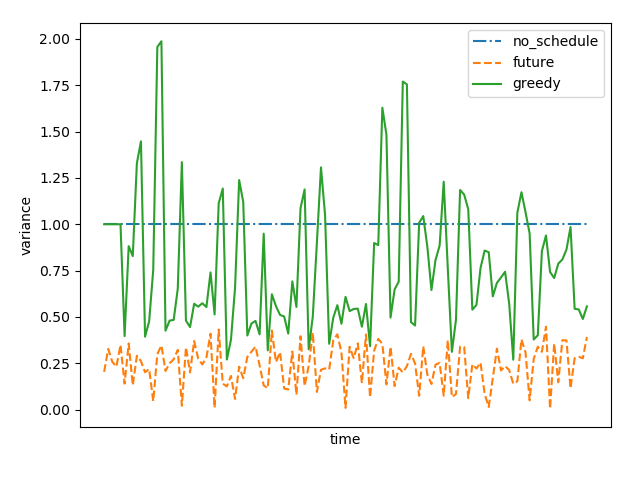
\includegraphics[width=0.4\textwidth]{Figure-3.2/Figure_1-1.png}
    \caption{Result of Simple Greedy Strategy on AY251Z}
    \label{fig3.2-1}
\end{figure}

For example, I/O pattern of many segments is periodic. In cluster AY251Z, the I/O pattern of a device, which has 16 segments and accounts for 9.2\% flow of the whole cluster, is in a cycle of 20 minutes. However, Figure \ref{fig3.2-2} indicates that these segments are in busy only in a short period of the cycle. If the observation range of history is too low, prediction will differ greatly from the actual state. However, if we raise the observation range, in some segments, local characteristics will be missed, though the periodic problem may be solved. As a result, average of historical records can not describe the pattern of the cluster properly. To improve the schedule result, detailed I/O pattern should be extracted for scheduling.


\begin{figure}[ht]
    \centering
    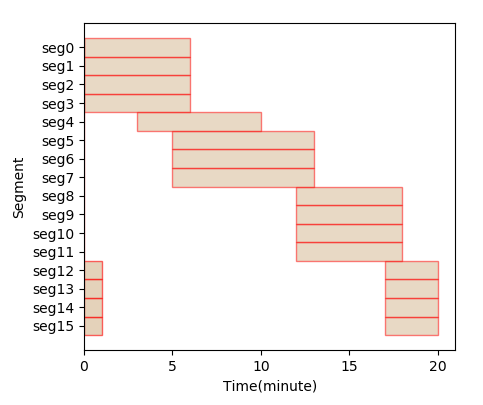
\includegraphics[width=0.4\textwidth]{Figure-3.2/Figure_2.png}
    \caption{Busy Time of Segments in a Certain Device}
    \label{fig3.2-2}
\end{figure}


\subsubsection{Impact of Knowledge of Future Throughput}
\label{sec3.2-3}

Scheduling effect not only depends on strategy itself, but also depends on the schedulability of the cluster. If we can know the future throughput of each segment, the scheduling effect will be improved. Hence, we can analyze the best case of greedy algorithms. We can use the following method to attempt to reach an approximate upper bound for any greedy schedule strategy. In the \textit{simple greedy strategy}, we pretend to know the future throughput of each segment, and execute scheduling with the future throughput. Besides, schedule should be frequent enough, or we will deviate from upper bound.

Table \ref{table3.2-1} shows the initial state and the approximate upper bound of any greedy algorithm. Note that, there is little potential for ESSD clusters to improve, while SSD clusters and efficient clusters have great potential to improve. As was stated in section \ref{sec3.1-3}, ESSD cloud disks have better performance and allow higher throughput. Thus, users are more likely to read and write more to the disk and the smallest unit of scheduling will be larger. This makes scheduling algorithm less effective on clusters with higher performance.


\subsubsection{Impact of Proportion of Segments to Schedule}
\label{sec3.2-4}

According to the 80/20 rule, we have a reason to believe that few segments contributes most to the variance of the entire cluster. Hence, we define a \textit{partial greedy strategy}, which only replace segments with the most throughput in each round of schedule. Evidently, the proportion of segments to schedule each time will also make an impact on the schedule result. Figure \ref{fig3.2-3} shows the relation between variance and the schedule proportion of \textit{partial greedy strategy}. Schedule interval and observation length of history are both 5 minutes.

\begin{figure}[ht]
    \centering
    \subfigure[AY336D]{
        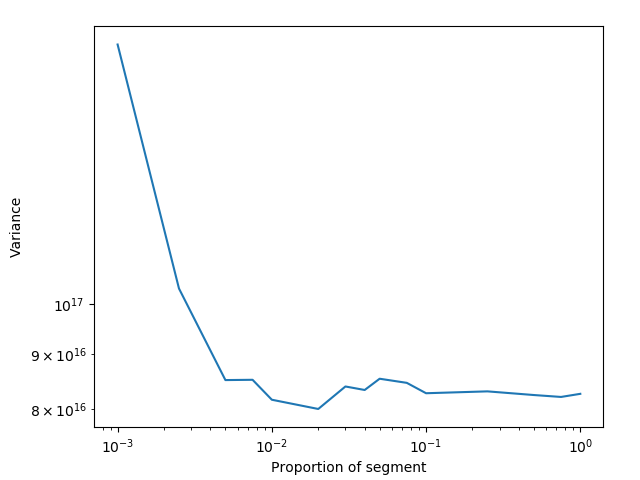
\includegraphics[width=1.45in]{Figure-3.2/Figure_3-AY336D.png}
    }
    \subfigure[AY272T]{
        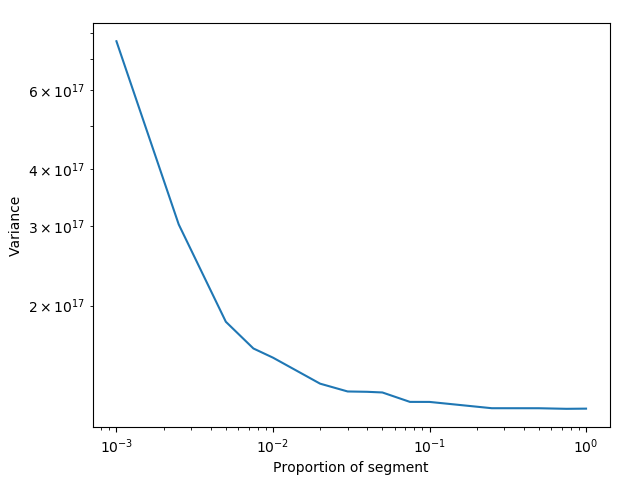
\includegraphics[width=1.45in]{Figure-3.2/Figure_3-AY272T.png}
    }
    
    \subfigure[AY306O]{
        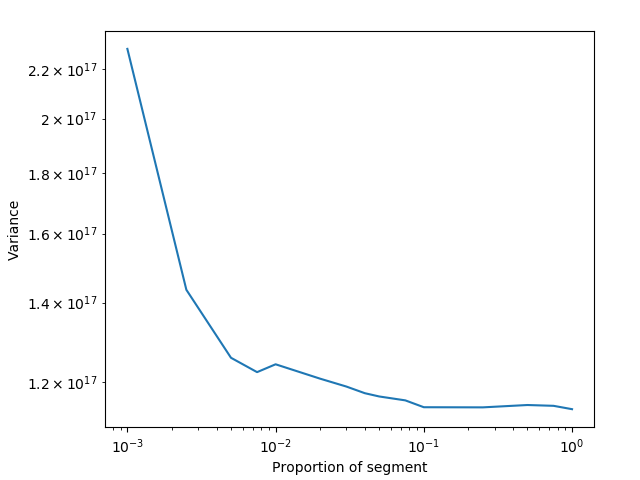
\includegraphics[width=1.45in]{Figure-3.2/Figure_3-AY306O.png}
    }
    \subfigure[AY251Z]{
        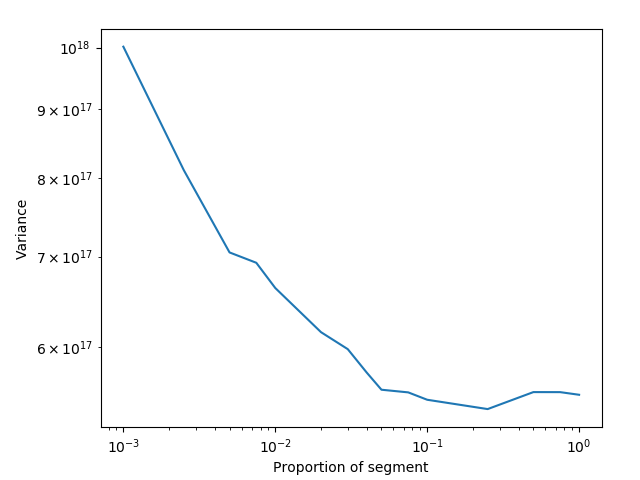
\includegraphics[width=1.45in]{Figure-3.2/Figure_3-AY251Z.png}
    }
    \centering
    \caption{Variance of Cluster with Different Schedule Proportion}
    \label{fig3.2-3}
\end{figure}

From the figure, we can learn that from the point of view of results, there is no significant difference between implementing greedy schedule for all the segments and for only 10\% of all segments. Few segments contributes most to the variance. Data from multiple clusters support this result.


% Use shows the following at camera-ready time to suppress page numbers.
% Comment it out when you first submit the paper for review.
%\thispagestyle{empty}

\bibliographystyle{acm}
\bibliography{references}

\end{document}
